% Options for packages loaded elsewhere
\PassOptionsToPackage{unicode}{hyperref}
\PassOptionsToPackage{hyphens}{url}
\PassOptionsToPackage{dvipsnames,svgnames,x11names}{xcolor}
%
\documentclass[
  letterpaper,
  DIV=11,
  numbers=noendperiod]{scrartcl}

\usepackage{amsmath,amssymb}
\usepackage{iftex}
\ifPDFTeX
  \usepackage[T1]{fontenc}
  \usepackage[utf8]{inputenc}
  \usepackage{textcomp} % provide euro and other symbols
\else % if luatex or xetex
  \usepackage{unicode-math}
  \defaultfontfeatures{Scale=MatchLowercase}
  \defaultfontfeatures[\rmfamily]{Ligatures=TeX,Scale=1}
\fi
\usepackage{lmodern}
\ifPDFTeX\else  
    % xetex/luatex font selection
\fi
% Use upquote if available, for straight quotes in verbatim environments
\IfFileExists{upquote.sty}{\usepackage{upquote}}{}
\IfFileExists{microtype.sty}{% use microtype if available
  \usepackage[]{microtype}
  \UseMicrotypeSet[protrusion]{basicmath} % disable protrusion for tt fonts
}{}
\makeatletter
\@ifundefined{KOMAClassName}{% if non-KOMA class
  \IfFileExists{parskip.sty}{%
    \usepackage{parskip}
  }{% else
    \setlength{\parindent}{0pt}
    \setlength{\parskip}{6pt plus 2pt minus 1pt}}
}{% if KOMA class
  \KOMAoptions{parskip=half}}
\makeatother
\usepackage{xcolor}
\setlength{\emergencystretch}{3em} % prevent overfull lines
\setcounter{secnumdepth}{5}
% Make \paragraph and \subparagraph free-standing
\makeatletter
\ifx\paragraph\undefined\else
  \let\oldparagraph\paragraph
  \renewcommand{\paragraph}{
    \@ifstar
      \xxxParagraphStar
      \xxxParagraphNoStar
  }
  \newcommand{\xxxParagraphStar}[1]{\oldparagraph*{#1}\mbox{}}
  \newcommand{\xxxParagraphNoStar}[1]{\oldparagraph{#1}\mbox{}}
\fi
\ifx\subparagraph\undefined\else
  \let\oldsubparagraph\subparagraph
  \renewcommand{\subparagraph}{
    \@ifstar
      \xxxSubParagraphStar
      \xxxSubParagraphNoStar
  }
  \newcommand{\xxxSubParagraphStar}[1]{\oldsubparagraph*{#1}\mbox{}}
  \newcommand{\xxxSubParagraphNoStar}[1]{\oldsubparagraph{#1}\mbox{}}
\fi
\makeatother

\usepackage{color}
\usepackage{fancyvrb}
\newcommand{\VerbBar}{|}
\newcommand{\VERB}{\Verb[commandchars=\\\{\}]}
\DefineVerbatimEnvironment{Highlighting}{Verbatim}{commandchars=\\\{\}}
% Add ',fontsize=\small' for more characters per line
\usepackage{framed}
\definecolor{shadecolor}{RGB}{241,243,245}
\newenvironment{Shaded}{\begin{snugshade}}{\end{snugshade}}
\newcommand{\AlertTok}[1]{\textcolor[rgb]{0.68,0.00,0.00}{#1}}
\newcommand{\AnnotationTok}[1]{\textcolor[rgb]{0.37,0.37,0.37}{#1}}
\newcommand{\AttributeTok}[1]{\textcolor[rgb]{0.40,0.45,0.13}{#1}}
\newcommand{\BaseNTok}[1]{\textcolor[rgb]{0.68,0.00,0.00}{#1}}
\newcommand{\BuiltInTok}[1]{\textcolor[rgb]{0.00,0.23,0.31}{#1}}
\newcommand{\CharTok}[1]{\textcolor[rgb]{0.13,0.47,0.30}{#1}}
\newcommand{\CommentTok}[1]{\textcolor[rgb]{0.37,0.37,0.37}{#1}}
\newcommand{\CommentVarTok}[1]{\textcolor[rgb]{0.37,0.37,0.37}{\textit{#1}}}
\newcommand{\ConstantTok}[1]{\textcolor[rgb]{0.56,0.35,0.01}{#1}}
\newcommand{\ControlFlowTok}[1]{\textcolor[rgb]{0.00,0.23,0.31}{\textbf{#1}}}
\newcommand{\DataTypeTok}[1]{\textcolor[rgb]{0.68,0.00,0.00}{#1}}
\newcommand{\DecValTok}[1]{\textcolor[rgb]{0.68,0.00,0.00}{#1}}
\newcommand{\DocumentationTok}[1]{\textcolor[rgb]{0.37,0.37,0.37}{\textit{#1}}}
\newcommand{\ErrorTok}[1]{\textcolor[rgb]{0.68,0.00,0.00}{#1}}
\newcommand{\ExtensionTok}[1]{\textcolor[rgb]{0.00,0.23,0.31}{#1}}
\newcommand{\FloatTok}[1]{\textcolor[rgb]{0.68,0.00,0.00}{#1}}
\newcommand{\FunctionTok}[1]{\textcolor[rgb]{0.28,0.35,0.67}{#1}}
\newcommand{\ImportTok}[1]{\textcolor[rgb]{0.00,0.46,0.62}{#1}}
\newcommand{\InformationTok}[1]{\textcolor[rgb]{0.37,0.37,0.37}{#1}}
\newcommand{\KeywordTok}[1]{\textcolor[rgb]{0.00,0.23,0.31}{\textbf{#1}}}
\newcommand{\NormalTok}[1]{\textcolor[rgb]{0.00,0.23,0.31}{#1}}
\newcommand{\OperatorTok}[1]{\textcolor[rgb]{0.37,0.37,0.37}{#1}}
\newcommand{\OtherTok}[1]{\textcolor[rgb]{0.00,0.23,0.31}{#1}}
\newcommand{\PreprocessorTok}[1]{\textcolor[rgb]{0.68,0.00,0.00}{#1}}
\newcommand{\RegionMarkerTok}[1]{\textcolor[rgb]{0.00,0.23,0.31}{#1}}
\newcommand{\SpecialCharTok}[1]{\textcolor[rgb]{0.37,0.37,0.37}{#1}}
\newcommand{\SpecialStringTok}[1]{\textcolor[rgb]{0.13,0.47,0.30}{#1}}
\newcommand{\StringTok}[1]{\textcolor[rgb]{0.13,0.47,0.30}{#1}}
\newcommand{\VariableTok}[1]{\textcolor[rgb]{0.07,0.07,0.07}{#1}}
\newcommand{\VerbatimStringTok}[1]{\textcolor[rgb]{0.13,0.47,0.30}{#1}}
\newcommand{\WarningTok}[1]{\textcolor[rgb]{0.37,0.37,0.37}{\textit{#1}}}

\providecommand{\tightlist}{%
  \setlength{\itemsep}{0pt}\setlength{\parskip}{0pt}}\usepackage{longtable,booktabs,array}
\usepackage{calc} % for calculating minipage widths
% Correct order of tables after \paragraph or \subparagraph
\usepackage{etoolbox}
\makeatletter
\patchcmd\longtable{\par}{\if@noskipsec\mbox{}\fi\par}{}{}
\makeatother
% Allow footnotes in longtable head/foot
\IfFileExists{footnotehyper.sty}{\usepackage{footnotehyper}}{\usepackage{footnote}}
\makesavenoteenv{longtable}
\usepackage{graphicx}
\makeatletter
\def\maxwidth{\ifdim\Gin@nat@width>\linewidth\linewidth\else\Gin@nat@width\fi}
\def\maxheight{\ifdim\Gin@nat@height>\textheight\textheight\else\Gin@nat@height\fi}
\makeatother
% Scale images if necessary, so that they will not overflow the page
% margins by default, and it is still possible to overwrite the defaults
% using explicit options in \includegraphics[width, height, ...]{}
\setkeys{Gin}{width=\maxwidth,height=\maxheight,keepaspectratio}
% Set default figure placement to htbp
\makeatletter
\def\fps@figure{htbp}
\makeatother

\usepackage{booktabs}
\usepackage{longtable}
\usepackage{array}
\usepackage{multirow}
\usepackage{wrapfig}
\usepackage{float}
\usepackage{colortbl}
\usepackage{pdflscape}
\usepackage{tabu}
\usepackage{threeparttable}
\usepackage{threeparttablex}
\usepackage[normalem]{ulem}
\usepackage{makecell}
\usepackage{xcolor}
\usepackage{caption}
\usepackage{anyfontsize}
\KOMAoption{captions}{tableheading}
\makeatletter
\@ifpackageloaded{float}{}{\usepackage{float}}
\floatstyle{plain}
\@ifundefined{c@chapter}{\newfloat{fig}{h}{lofig}}{\newfloat{fig}{h}{lofig}[chapter]}
\floatname{fig}{Figure}
\newcommand*\listoffigs{\listof{fig}{List of Figures}}
\makeatother
\makeatletter
\@ifpackageloaded{float}{}{\usepackage{float}}
\floatstyle{plain}
\@ifundefined{c@chapter}{\newfloat{suppfig}{h}{losuppfig}}{\newfloat{suppfig}{h}{losuppfig}[chapter]}
\floatname{suppfig}{Supplementary Figure}
\newcommand*\listofsuppfigs{\listof{suppfig}{List of Supplementary Figures}}
\makeatother
\makeatletter
\@ifpackageloaded{float}{}{\usepackage{float}}
\floatstyle{plain}
\@ifundefined{c@chapter}{\newfloat{tbl}{h}{lotbl}}{\newfloat{tbl}{h}{lotbl}[chapter]}
\floatname{tbl}{Table}
\newcommand*\listoftbls{\listof{tbl}{List of Tables}}
\makeatother
\makeatletter
\@ifpackageloaded{float}{}{\usepackage{float}}
\floatstyle{plain}
\@ifundefined{c@chapter}{\newfloat{supptbl}{h}{losupptbl}}{\newfloat{supptbl}{h}{losupptbl}[chapter]}
\floatname{supptbl}{Supplementary Table}
\newcommand*\listofsupptbls{\listof{supptbl}{List of Supplementary Tables}}
\makeatother
\makeatletter
\@ifpackageloaded{caption}{}{\usepackage{caption}}
\AtBeginDocument{%
\ifdefined\contentsname
  \renewcommand*\contentsname{Table of contents}
\else
  \newcommand\contentsname{Table of contents}
\fi
\ifdefined\listfigurename
  \renewcommand*\listfigurename{List of Figures}
\else
  \newcommand\listfigurename{List of Figures}
\fi
\ifdefined\listtablename
  \renewcommand*\listtablename{List of Tables}
\else
  \newcommand\listtablename{List of Tables}
\fi
\ifdefined\figurename
  \renewcommand*\figurename{Figure}
\else
  \newcommand\figurename{Figure}
\fi
\ifdefined\tablename
  \renewcommand*\tablename{Table}
\else
  \newcommand\tablename{Table}
\fi
}
\@ifpackageloaded{float}{}{\usepackage{float}}
\floatstyle{ruled}
\@ifundefined{c@chapter}{\newfloat{codelisting}{h}{lop}}{\newfloat{codelisting}{h}{lop}[chapter]}
\floatname{codelisting}{Listing}
\newcommand*\listoflistings{\listof{codelisting}{List of Listings}}
\makeatother
\makeatletter
\makeatother
\makeatletter
\@ifpackageloaded{caption}{}{\usepackage{caption}}
\@ifpackageloaded{subcaption}{}{\usepackage{subcaption}}
\makeatother

\ifLuaTeX
  \usepackage{selnolig}  % disable illegal ligatures
\fi
\usepackage{bookmark}

\IfFileExists{xurl.sty}{\usepackage{xurl}}{} % add URL line breaks if available
\urlstyle{same} % disable monospaced font for URLs
\hypersetup{
  pdftitle={Pika-Yak Interaction: Plant Cover},
  pdfauthor={Douglas Lawton},
  colorlinks=true,
  linkcolor={blue},
  filecolor={Maroon},
  citecolor={Blue},
  urlcolor={Blue},
  pdfcreator={LaTeX via pandoc}}


\title{Pika-Yak Interaction: Plant Cover}
\author{Douglas Lawton}
\date{2025-09-01}

\begin{document}
\maketitle

\renewcommand*\contentsname{Table of contents}
{
\hypersetup{linkcolor=}
\setcounter{tocdepth}{3}
\tableofcontents
}

\begin{fig}

\centering{

::: \{.cell\}

\begin{Shaded}
\begin{Highlighting}[]
\FunctionTok{library}\NormalTok{(cowplot)}
\end{Highlighting}
\end{Shaded}

::: \{.cell-output .cell-output-stderr\}

\begin{verbatim}

Attaching package: 'cowplot'
\end{verbatim}

:::

::: \{.cell-output .cell-output-stderr\}

\begin{verbatim}
The following object is masked from 'package:gt':

    as_gtable
\end{verbatim}

:::

::: \{.cell-output .cell-output-stderr\}

\begin{verbatim}
The following object is masked from 'package:patchwork':

    align_plots
\end{verbatim}

:::

::: \{.cell-output .cell-output-stderr\}

\begin{verbatim}
The following object is masked from 'package:ggpubr':

    get_legend
\end{verbatim}

:::

::: \{.cell-output .cell-output-stderr\}

\begin{verbatim}
The following object is masked from 'package:lubridate':

    stamp
\end{verbatim}

:::

\begin{Shaded}
\begin{Highlighting}[]
\FunctionTok{library}\NormalTok{(magick)}
\end{Highlighting}
\end{Shaded}

::: \{.cell-output .cell-output-stderr\}

\begin{verbatim}
Linking to ImageMagick 7.1.2.3
Enabled features: fontconfig, freetype, heic, lcms, raw, webp
Disabled features: cairo, fftw, ghostscript, pango, rsvg, x11
\end{verbatim}

:::

::: \{.cell-output .cell-output-stderr\}

\begin{verbatim}
Using 7 threads
\end{verbatim}

:::

\begin{Shaded}
\begin{Highlighting}[]
\NormalTok{hypoth\_pic }\OtherTok{\textless{}{-}}\NormalTok{ png}\SpecialCharTok{::}\FunctionTok{readPNG}\NormalTok{(}\FunctionTok{here}\NormalTok{(}\StringTok{\textquotesingle{}data/photos/hypothesis\_figure.png\textquotesingle{}}\NormalTok{))}
\NormalTok{hypoth\_pic }\OtherTok{\textless{}{-}} \FunctionTok{ggdraw}\NormalTok{() }\SpecialCharTok{+} \FunctionTok{draw\_image}\NormalTok{(hypoth\_pic) }\SpecialCharTok{+} \FunctionTok{theme\_void}\NormalTok{(}\AttributeTok{base\_size=}\DecValTok{15}\NormalTok{)}

\NormalTok{hypoth\_pic}
\end{Highlighting}
\end{Shaded}

::: \{.cell-output-display\}
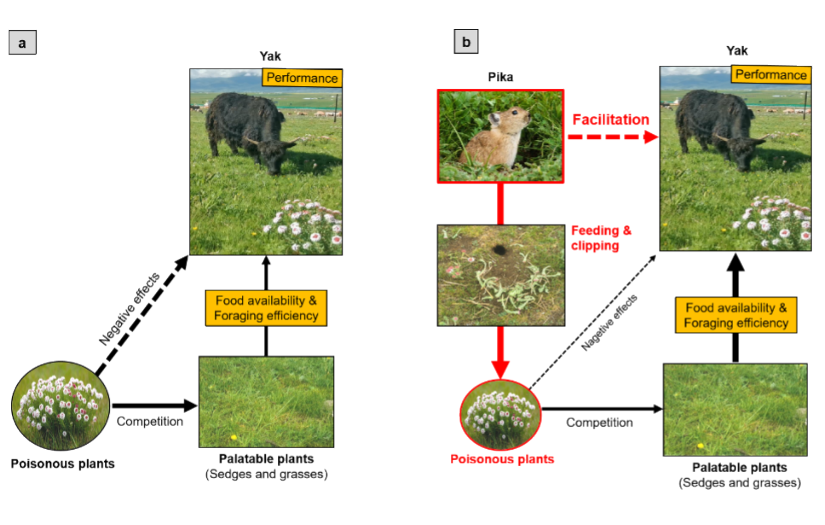
\includegraphics{manuscript_figures_and_text_files/figure-pdf/hypothesis figure-1.pdf}
::: :::

}

\caption{\label{fig-hypothesis}The hypothesized facilitative effects of
pika on yak in the Tibetan Plateau. In the absence of pika, the
poisonous Stellera chamaejasme forbs should exert a strong negative
effect on yak growth performance by competing with the palatable grasses
and sedges, decreasing their food availability and foraging efficiency
(Fig. 1a). However, such negative effects of poisonous plants should be
mitigated in the presence of pika, whom eliminate S. chamaejasme forbs
by their feeding and clipping activities, leading to a facilitative
effect on yak (Fig. 1b). The negative effects of poisonous plants on yak
were indicated as black dashed lines, the competition between plant
groups were indicated by the black solid lines, and the pathway that
pika suppress poisonous plants was indicated by red solid line. The
sizes of the lines indicate the strengths of species interactions.
Credits: Xiaona Zheng (photographs).}

\end{fig}%

\section{Methods}\label{methods}

\subsection{Statistical analyses}\label{statistical-analyses}

All data were analyzed using linear models, generalized linear mixed
models, or generalized additive models, with the choice of model and
statistical family guided by the structure and distribution of the data.
Posthoc comparisons were conducted only when the pika × S. chamaejasme
interaction term was significant. For the 2021 field surveys, we fit
generalized linear mixed models with plot and month as random effects.
We then used generalized additive mixed models for S. chamaejasme cover
and active pika burrow density, with plot as a random effect, and linear
regression models for dung density and S. chamaejasme cover. For the
field manipulation experiments in 2022 and 2023, we constructed
generalized linear mixed models with the dependent variables (e.g.,
grass bites per step, sedge total bites, weight gain) regressed against
the interactive effect of pika and S. chamaejasme treatments, while
including block, year, and month as random effects to capture the
hierarchical structure of the data. Models assumed gaussian, beta (for
proportions), or tweedie (for non-normal data) distributions, selected
based on data type and model fit. A significance threshold of P = 0.05
was applied, with TukeyHSD or Sidak posthoc tests used where
appropriate. All data management, modeling, and visualization were
carried out in R, with dependencies managed using \emph{renv}. The main
modeling packages were \emph{glmmTMB} and \emph{mgcv}, with
\emph{DHARMa} used for model diagnostics. Data management relied on the
\emph{tidyverse} suite of packages. A complete record of package
versions is available in the renv.lock file in the repository:
\url{https://github.com/ddlawton/pika_yak_interactions}.

\section{Results and Discussion}\label{results-and-discussion}

First, we carried out a set of field observational experiments to
investigate diet selection by pika and yak, as well as the associations
among pika abundance, S. chamaejasme abundance, and yak activity under
natural field conditions. Consistent with previous
studies\textsuperscript{5,11,24--25}, we found that pika and yak have
distinct diet preferences: yaks preferred grasses and sedges, while pika
preferred the poisonous S. chamaejasme (Figure~\ref{fig-diet-selection}
A,B, Supplementary Table~\ref{supptbl-pika-yak-feeding-model-summary},
Supplementary Table~\ref{supptbl-pika-yak-feeding-model-contrast}). We
also found that S. chamaejasme abundance was negatively associated with
active pika burrow abundance (Figure~\ref{fig-diet-selection} C) and
with yak foraging activity, as indicated by dung density
(Figure~\ref{fig-diet-selection} D).

Building on these results, we conducted an in-situ manipulative field
experiment using fenced enclosures to test the interactive effects of
pika and S. chamaejasme on yak weight gain, foraging quantity and
quality, and grazing behavior. For weight gain, yaks gained less in
poison-plant plots than in non-poison plots, and there was a significant
interaction between pika and S. chamaejasme treatments
(Supplementary Table~\ref{supptbl-yak-performance-model-summary}). When
pika were present, yaks showed higher weight gain
(Supplementary Table~\ref{supptbl-yak-performance-model-contrast}). This
effect was driven by pika feeding on S. chamaejasme
(Figure~\ref{fig-diet-selection} B,
Supplementary Table~\ref{supptbl-yak-performance-model-summary},
Supplementary Table~\ref{supptbl-yak-performance-model-contrast}), which
increased grass cover (Figure~\ref{fig-diet-selection} C,
Supplementary Table~\ref{supptbl-yak-performance-model-summary},
Supplementary Table~\ref{supptbl-yak-performance-model-contrast})
compared to plots with S. chamaejasme but no pika.

Food quantity and quality are key drivers of individual performance and
population dynamics in large herbivores\textsuperscript{30--32}. In the
presence of \emph{S. chamaejasme} forbs, pika doubled the cover of yak's
most preferred grasses (Figure~\ref{fig-diet-selection} C,
Supplementary Table~\ref{supptbl-yak-performance-model-summary},
Supplementary Table~\ref{supptbl-yak-performance-model-contrast}) and
increased the crude protein content of total forage by approximately
16\% (Figure~\ref{fig-yak-performance} D,
Supplementary Table~\ref{supptbl-yak-performance-model-summary},
Supplementary Table~\ref{supptbl-yak-performance-model-contrast}),
suggesting that pika facilitate yak by enhancing both the quantity and
quality of forage. Acid detergent fibre (6\%) was higher in pika plots,
while ether extract also differed significantly between treatments
(Figure~\ref{fig-yak-performance} E,F,
Supplementary Table~\ref{supptbl-yak-performance-model-summary},
Supplementary Table~\ref{supptbl-yak-performance-model-contrast}). These
increases in grass abundance and forage quality were likely driven by
the decline in poisonous plants induced by pika
(Figure~\ref{fig-yak-performance} B), which reduced interspecific
competition for shared resources (e.g., light, soil moisture, nutrients)
and allowed grasses to expand\textsuperscript{27--28}. In the absence of
S. chamaejasme forbs, however, the positive effects of pika on food
resources and yak weight gain disappeared
(Figure~\ref{fig-yak-performance} A,C,D). Pika and poisonous plants
influenced sedge cover in a similar way as grass cover
(Supplementary Figure~\ref{suppfig-other-figs} A), while interactions
with forb cover were more complex
(Supplementary Figure~\ref{suppfig-other-figs} B). There was no impact
of pika or poisonous plants on neutral detergent fibre
(Supplementary Figure~\ref{suppfig-other-figs} C).

Pika-yak facilitation was also linked to improved foraging efficiency in
yak when grazing alongside pika. Optimal foraging theory predicts that
animals minimize energy costs to exploit high-quality food items and
maximize intake of digestible nutrients, thereby improving
performance\textsuperscript{33}. In ruminants, bite rate, step rate, and
bites per step are key predictors of foraging
efficiency\textsuperscript{34} and, ultimately, animal
performance\textsuperscript{35}. In the presence of \emph{S.
chamaejasme} forbs, yak total, sedge, and grass bite rates increased by
roughly 35\% (Figure~\ref{fig-yak-foraging-efficiency} A), 48\%
(Figure~\ref{fig-yak-foraging-efficiency} B), and 41\%
(Figure~\ref{fig-yak-foraging-efficiency} C), respectively, in the
treatment where they coexisted with pika
(Supplementary Table~\ref{supptbl-yak-foraging-efficiency-summary},
Supplementary Table~\ref{supptbl-yak-foraging-efficiency-contrast}). Yak
stepped more often in the presence of \emph{S. chamaejasme} forbs
without pika, which meant they consumed more grasses and sedges per step
in plots where pika were present.

Yak total steps were also higher in the presence of \emph{S.
chamaejasme} forbs when pika were absent
(Figure~\ref{fig-yak-foraging-efficiency} D). In contrast, sedge bites
per step and grass bites per step increased significantly by r
\{sedge\_bite\_steps\}\% (Figure~\ref{fig-yak-foraging-efficiency} E)
and 41\% (Figure~\ref{fig-yak-performance} F) in plots with pika. These
gains in foraging efficiency can be attributed to the decline in
\emph{S. chamaejasme} forbs (Figure~\ref{fig-yak-performance} B), which
improved access to palatable grasses and sedges. In this system,
increased food availability (Figure~\ref{fig-yak-performance} C,D) and
enhanced foraging efficiency (Figure~\ref{fig-yak-performance}) likely
work together to shape the facilitative effects of pika on yak
performance (Figure~\ref{fig-yak-performance} A).

\begin{fig}

\centering{

\centering{

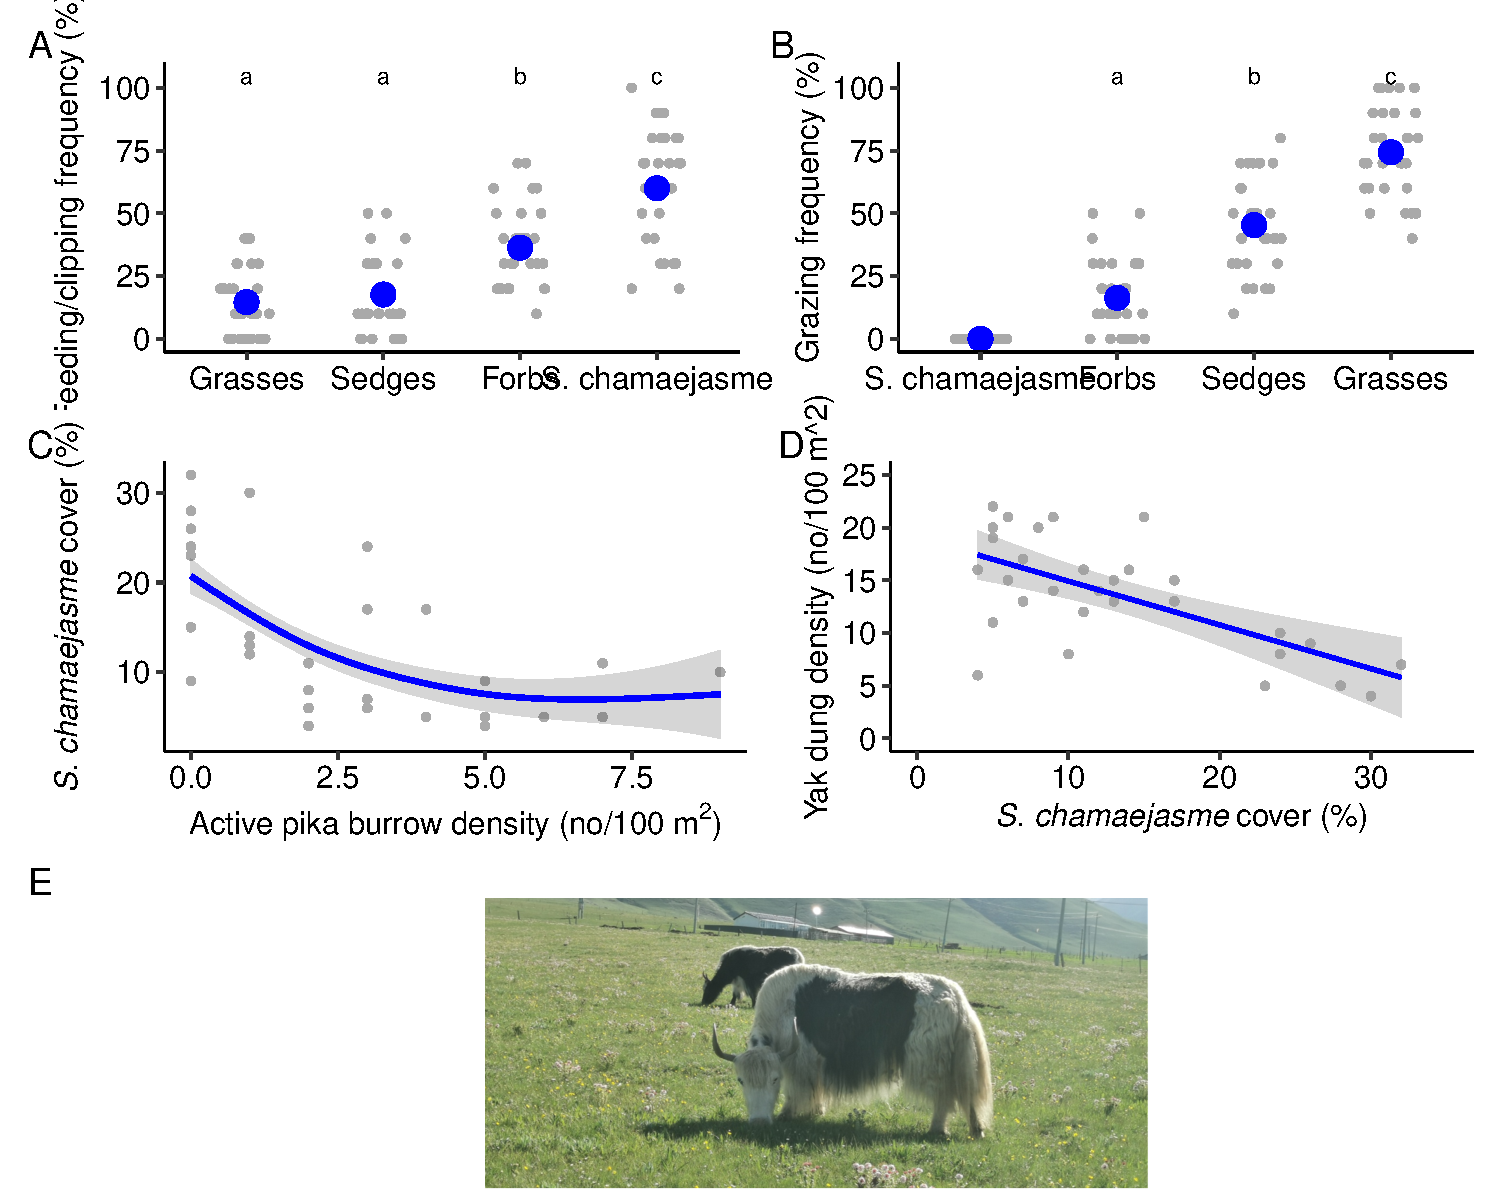
\includegraphics{manuscript_figures_and_text_files/figure-pdf/fig-diet-selection-1.pdf}

}

\subcaption{\label{fig-diet-selection}}

}

\caption{\label{fig-diet-selection}Diet selection of pika and yak and
their potential interactions mediated by poisonous plants in the field
surveys in July 2021. (a) Feeding and clipping frequency of pika, and
(b) grazing frequency of yak on the S. chamaejasme, sedges, grasses, and
forbs in the 10 2 m × 2 m plots and the 10 250 m transects,
respectively. (c) The relationship between active pika burrow density
and S. chamaejasme cover, and (d) the relationship between S.
chamaejasme cover and yak grazing activity in the 30 10 m × 10 m plots.
(e) Two yak were grazing around the poisonous S. chamaejasme during its
flowering season (i.e., May to June) in the study site. Different
letters above the bars indicate significant differences at P \textless{}
0.05.}

\end{fig}%

\begin{fig}

\centering{

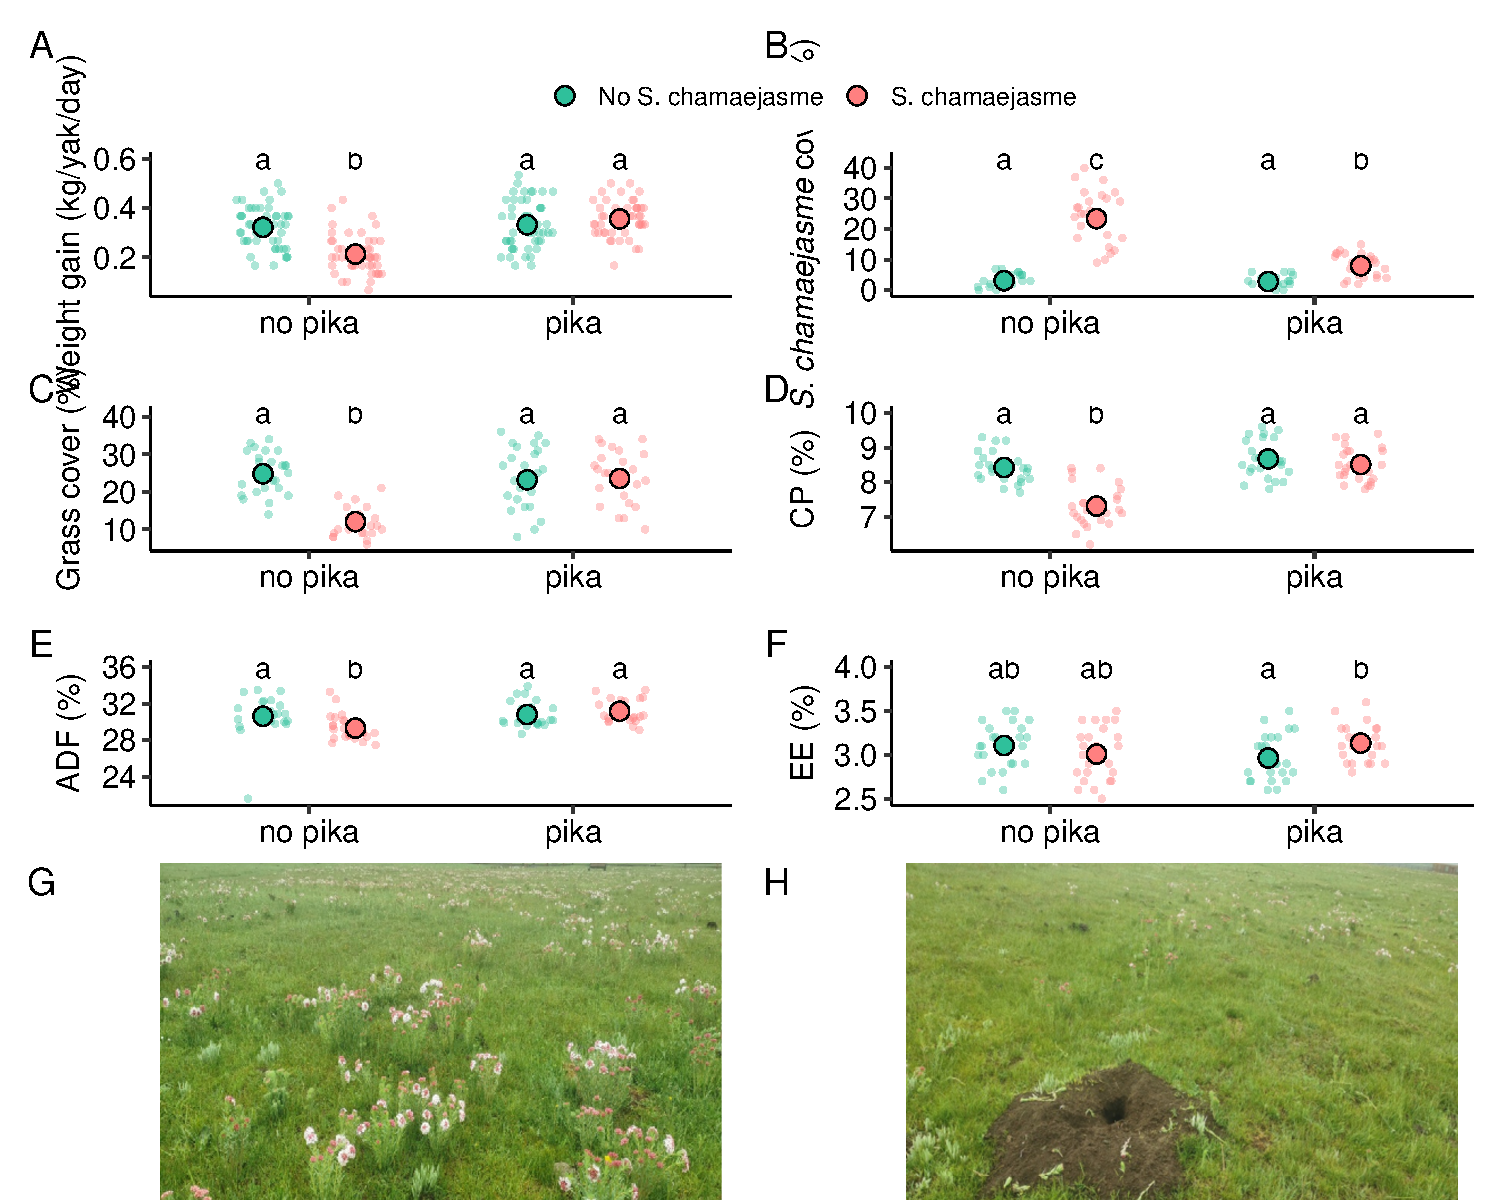
\includegraphics{manuscript_figures_and_text_files/figure-pdf/unnamed-chunk-1-1.pdf}

}

\caption{\label{fig-yak-performance}Combined effects of 2-yr (2022-2023)
pika and poisonous plant removal treatments on yak performance, forage
quantity and quality in the field manipulated experiments. (a) yak
weight gain, (b) S. chamaejasme cover, (c) grass cover, and (d) crude
protein (CP) content of total forage based on dry mass. The average
values of each variable in the two years were used for statistical
analysis, providing a single data point for each variable in each 150 m
× 150 m plot. (e) and (f) Show how S. chamaejasme abundance respond to
the absence and presence of pika, respectively. Significant interactions
between pika and S. chamaejasme plants were evaluated with post hoc
comparisons; means that do not share letters are significantly
different. Error bars represent +/- SE.}

\end{fig}%

\begin{fig}

\centering{

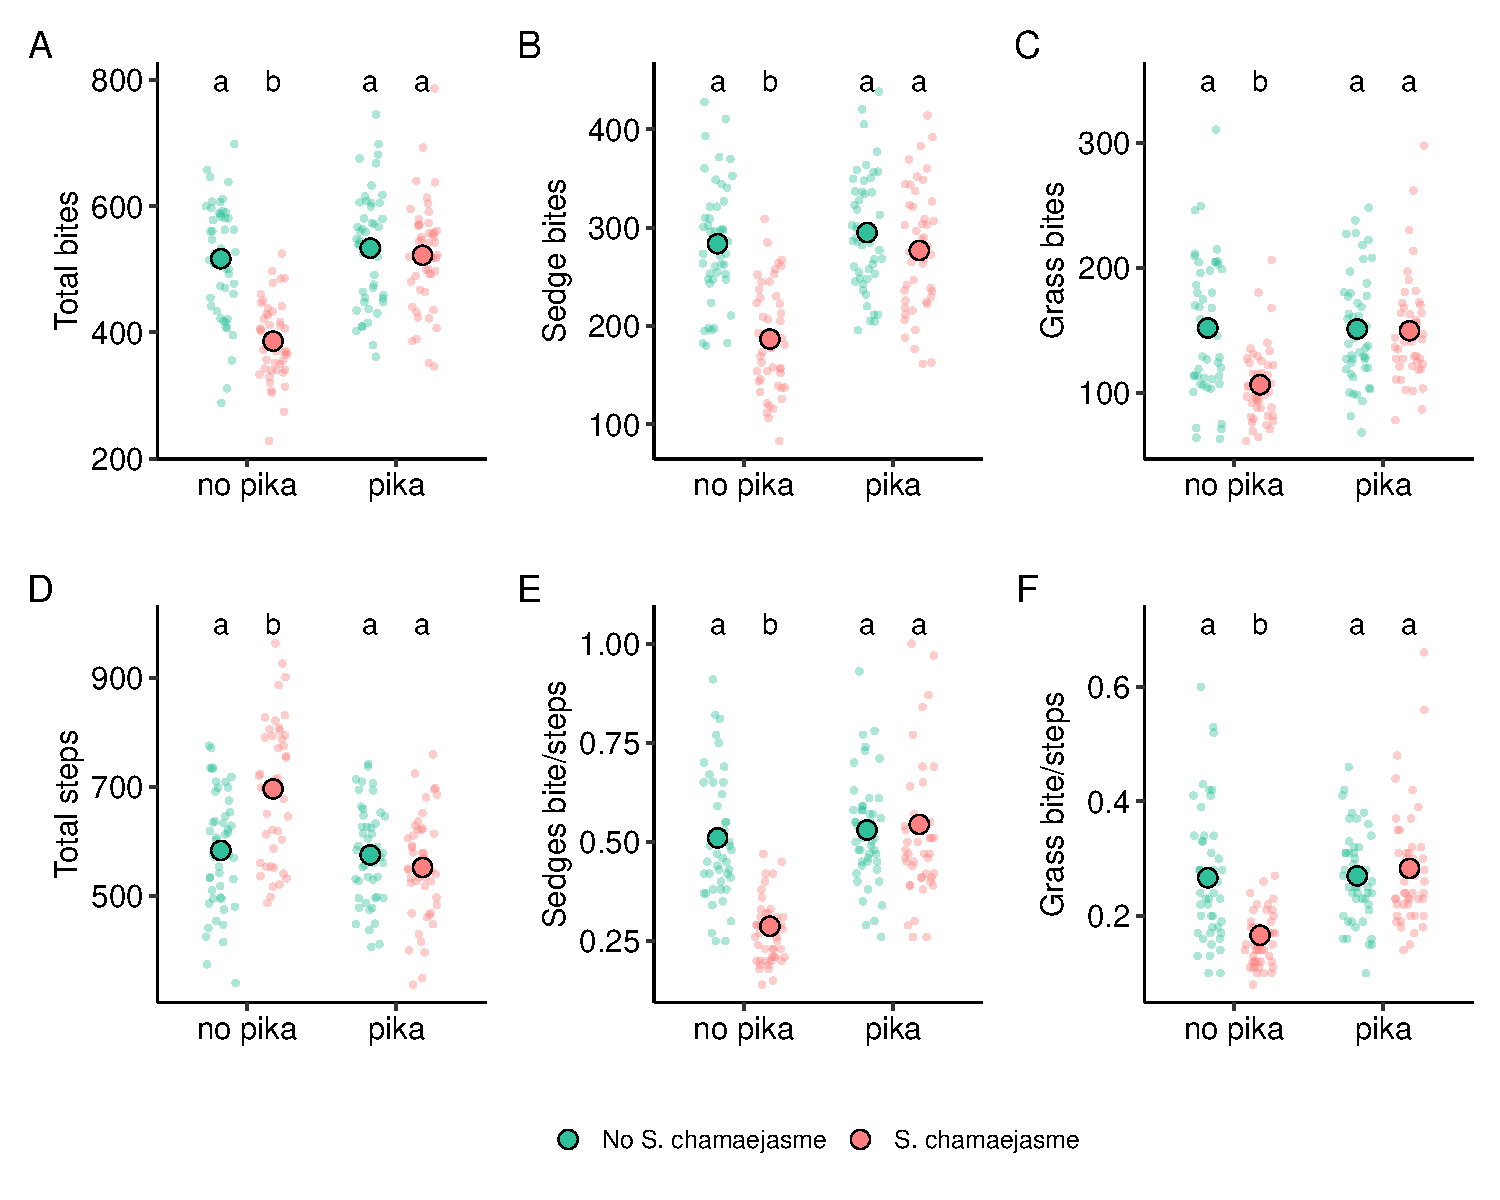
\includegraphics{manuscript_figures_and_text_files/figure-pdf/fig-yak-foraging-efficiency-1.pdf}

}

\caption{\label{fig-yak-foraging-efficiency}Combined effects of 2-yr
(2022-2023) pika and poisonous plant removal treatments on foraging
efficiency of yak in the field manipulated experiments. (a) Total bite
rate, (b) sedge bite rate, (c) grass bite rate, (d) total step rate, (e)
sedge bites per step, and (f) grass bites per step. The average values
of each variable in the two years were used for statistical analysis,
providing a single data point for each variable in each 150 m × 150 m
plot. Significant interactions between pika and S. chamaejasme plants
were evaluated with post hoc comparisons; means that do not share
letters are significantly different. Error bars represent +/- SE.}

\end{fig}%

\section{Supplementary Figures and
Tables}\label{supplementary-figures-and-tables}

\begin{suppfig}

\centering{

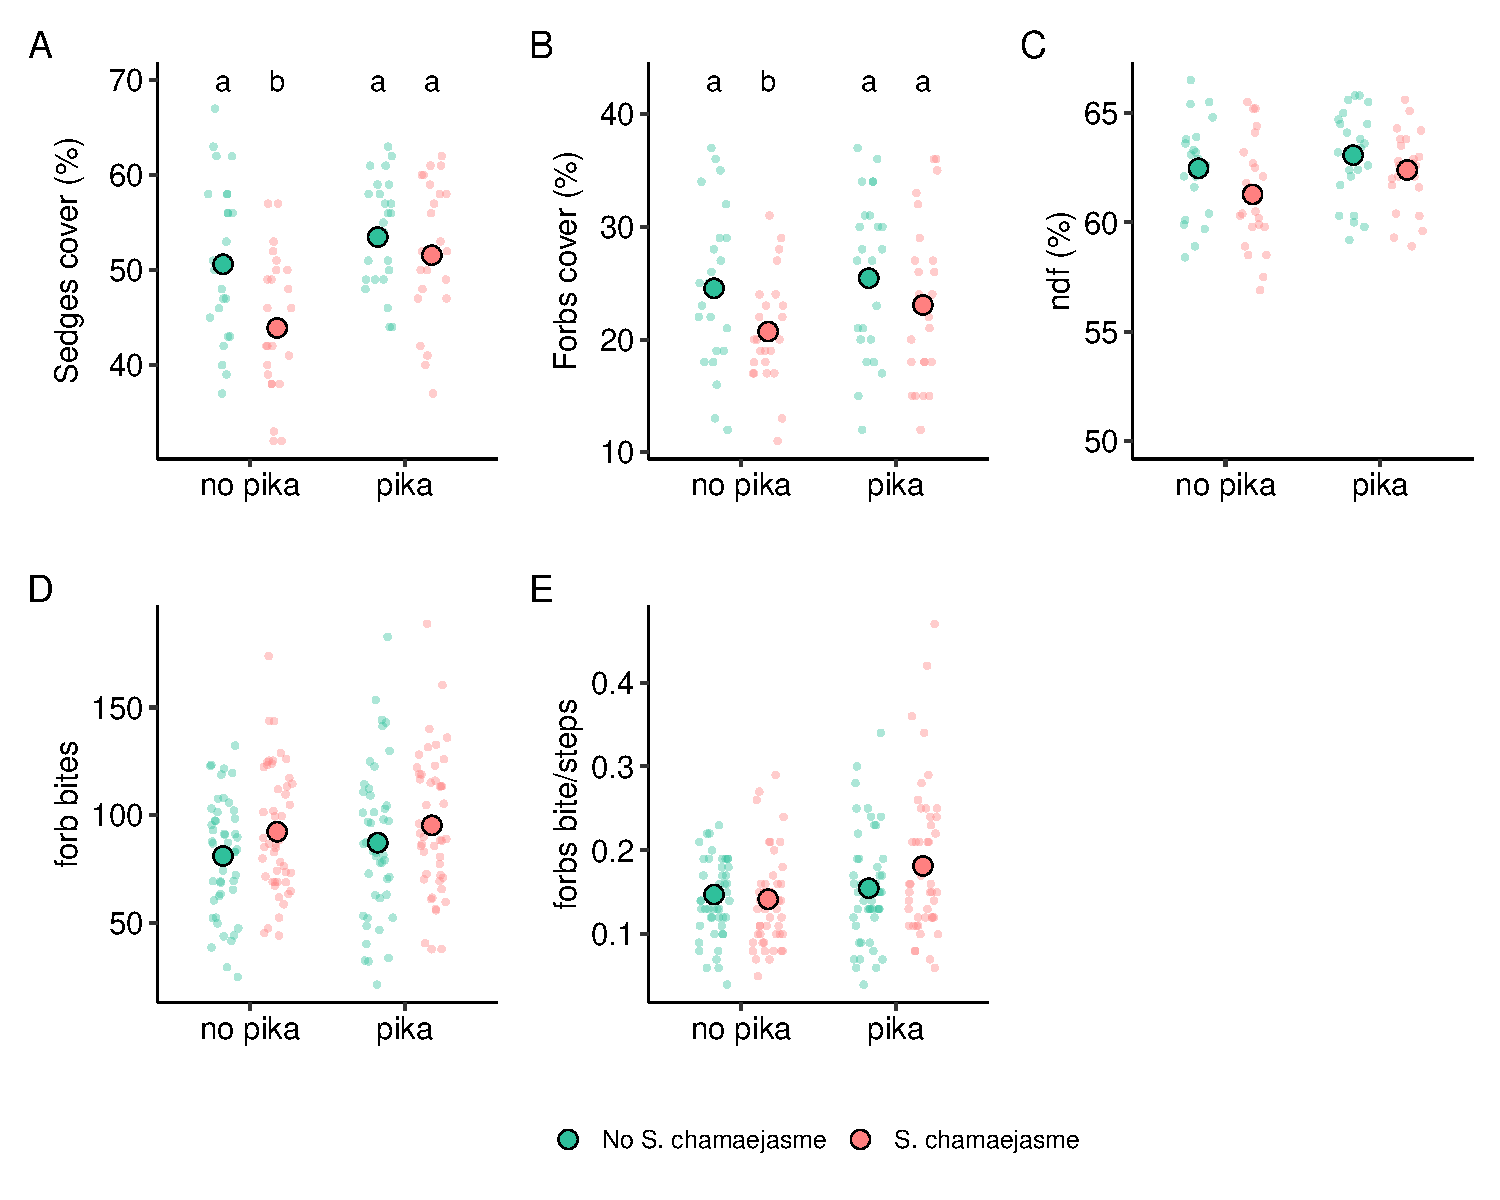
\includegraphics{manuscript_figures_and_text_files/figure-pdf/suppfig-other-figs-1.pdf}

}

\caption{\label{suppfig-other-figs}Sedge cover percent (A), forb cover
percent (B), ndf percent, total plant yak bites, and yak plant
bite/steps by pika and \emph{S. chamaejasme} treatment. Sedge cover was
lower in no pika and \emph{S. chamaejasme} plots than any other
treatment level and there was a trending decrease in forb cover as well.
in the same plot, but it was not significantly different from no pika,
no \emph{S. chamaejasme} plots and pika, \emph{S. chamaejasme} plots.\\
There was no signficant different in the interaction between pika and
\emph{S. chamaejasme} treatments for NDF, yak forb bite, and yak forb
bite/step.}

\end{suppfig}%

\begin{supptbl}

\centering{

\begin{table}
\fontsize{12.0pt}{14.4pt}\selectfont
\begin{tabular*}{\linewidth}{@{\extracolsep{\fill}}llrrrr}
\toprule
effect & term & estimate & std.error & statistic & p.value \\ 
\midrule\addlinespace[2.5pt]
\multicolumn{6}{l}{Pika feeding} \\[2.5pt] 
\midrule\addlinespace[2.5pt]
fixed & (Intercept) & 36.33 & 3.24 & 11.23 & 0.00 \\ 
fixed & Grasses & -21.67 & 4.39 & -4.94 & 0.00 \\ 
fixed & S. chamaejasme & 23.67 & 4.39 & 5.39 & 0.00 \\ 
fixed & Sedges & -18.67 & 4.39 & -4.25 & 0.00 \\ 
random & plot & 0.00 & NA & NA & NA \\ 
random & month & 1.58 & NA & NA & NA \\ 
random & Residual & 17.00 & NA & NA & NA \\ 
\midrule\addlinespace[2.5pt]
\multicolumn{6}{l}{Yak feeding} \\[2.5pt] 
\midrule\addlinespace[2.5pt]
fixed & (Intercept) & 16.33 & 3.23 & 5.05 & 0.00 \\ 
fixed & Grasses & 58.00 & 4.24 & 13.68 & 0.00 \\ 
fixed & Sedges & 29.00 & 4.24 & 6.84 & 0.00 \\ 
random & transect & 3.83 & NA & NA & NA \\ 
random & month & 0.00 & NA & NA & NA \\ 
random & Residual & 16.42 & NA & NA & NA \\ 
\bottomrule
\end{tabular*}
\end{table}

}

\caption{\label{supptbl-pika-yak-feeding-model-summary}Model summary for
pika and yak feeding.}

\end{supptbl}%

\begin{supptbl}

\centering{

\begin{table}
\fontsize{12.0pt}{14.4pt}\selectfont
\begin{tabular*}{\linewidth}{@{\extracolsep{\fill}}lrrrrr}
\toprule
contrast & estimate & SE & df & t.ratio & p.value \\ 
\midrule\addlinespace[2.5pt]
\multicolumn{6}{l}{Pika feeding} \\[2.5pt] 
\midrule\addlinespace[2.5pt]
Forbs - Grasses & 21.67 & 4.39 & 113.00 & 4.94 & 0.00 \\ 
Forbs - S. chamaejasme & -23.67 & 4.39 & 113.00 & -5.39 & 0.00 \\ 
Forbs - Sedges & 18.67 & 4.39 & 113.00 & 4.25 & 0.00 \\ 
Grasses - S. chamaejasme & -45.33 & 4.39 & 113.00 & -10.33 & 0.00 \\ 
Grasses - Sedges & -3.00 & 4.39 & 113.00 & -0.68 & 0.90 \\ 
S. chamaejasme - Sedges & 42.33 & 4.39 & 113.00 & 9.64 & 0.00 \\ 
\midrule\addlinespace[2.5pt]
\multicolumn{6}{l}{Yak feeding} \\[2.5pt] 
\midrule\addlinespace[2.5pt]
Forbs - Grasses & -58.00 & 4.24 & 84.00 & -13.68 & 0.00 \\ 
Forbs - Sedges & -29.00 & 4.24 & 84.00 & -6.84 & 0.00 \\ 
Grasses - Sedges & 29.00 & 4.24 & 84.00 & 6.84 & 0.00 \\ 
\bottomrule
\end{tabular*}
\end{table}

}

\caption{\label{supptbl-pika-yak-feeding-model-contrast}Model contrasts
for pika and yak feeding.}

\end{supptbl}%

\begin{supptbl}

\centering{

\begin{table}
\fontsize{12.0pt}{14.4pt}\selectfont
\begin{tabular*}{\linewidth}{@{\extracolsep{\fill}}llrrrr}
\toprule
effect & term & estimate & std.error & statistic & p.value \\ 
\midrule\addlinespace[2.5pt]
\multicolumn{6}{l}{weight gain} \\[2.5pt] 
\midrule\addlinespace[2.5pt]
fixed & (Intercept) & 0.32 & 0.03 & 10.80 & 0.00 \\ 
fixed & pika & 0.01 & 0.01 & 0.74 & 0.46 \\ 
fixed & S. chamaejasme & -0.11 & 0.01 & -7.70 & 0.00 \\ 
fixed & pika:S. chamaejasme & 0.13 & 0.02 & 6.63 & 0.00 \\ 
random & block & 0.01 & NA & NA & NA \\ 
random & year & 0.01 & NA & NA & NA \\ 
random & month & 0.05 & NA & NA & NA \\ 
random & Residual & 0.07 & NA & NA & NA \\ 
\midrule\addlinespace[2.5pt]
\multicolumn{6}{l}{grass cover} \\[2.5pt] 
\midrule\addlinespace[2.5pt]
fixed & (Intercept) & -1.11 & 0.10 & -11.58 & 0.00 \\ 
fixed & pika & -0.09 & 0.10 & -0.90 & 0.37 \\ 
fixed & S. chamaejasme & -0.88 & 0.11 & -7.76 & 0.00 \\ 
fixed & pika:S. chamaejasme & 0.90 & 0.15 & 5.97 & 0.00 \\ 
random & block & 0.13 & NA & NA & NA \\ 
random & year & 0.00 & NA & NA & NA \\ 
random & month & 0.02 & NA & NA & NA \\ 
\midrule\addlinespace[2.5pt]
\multicolumn{6}{l}{S. chamaejasme} \\[2.5pt] 
\midrule\addlinespace[2.5pt]
fixed & (Intercept) & -3.44 & 0.26 & -13.39 & 0.00 \\ 
fixed & pika & -0.11 & 0.22 & -0.49 & 0.62 \\ 
fixed & S. chamaejasme & 2.25 & 0.17 & 12.91 & 0.00 \\ 
fixed & pika:S. chamaejasme & -1.15 & 0.25 & -4.58 & 0.00 \\ 
random & block & 0.16 & NA & NA & NA \\ 
random & year & 0.17 & NA & NA & NA \\ 
random & month & 0.24 & NA & NA & NA \\ 
\midrule\addlinespace[2.5pt]
\multicolumn{6}{l}{crude protein \%} \\[2.5pt] 
\midrule\addlinespace[2.5pt]
fixed & (Intercept) & -2.39 & 0.02 & -107.03 & 0.00 \\ 
fixed & pika & 0.03 & 0.02 & 1.88 & 0.06 \\ 
fixed & S. chamaejasme & -0.15 & 0.02 & -8.72 & 0.00 \\ 
fixed & pika:S. chamaejasme & 0.13 & 0.02 & 5.45 & 0.00 \\ 
random & block & 0.01 & NA & NA & NA \\ 
random & year & 0.00 & NA & NA & NA \\ 
random & month & 0.03 & NA & NA & NA \\ 
\midrule\addlinespace[2.5pt]
\multicolumn{6}{l}{acid detergent fibre \%} \\[2.5pt] 
\midrule\addlinespace[2.5pt]
fixed & (Intercept) & -0.82 & 0.03 & -32.36 & 0.00 \\ 
fixed & pika & 0.01 & 0.02 & 0.46 & 0.65 \\ 
fixed & S. chamaejasme & -0.06 & 0.02 & -3.14 & 0.00 \\ 
fixed & pika:S. chamaejasme & 0.08 & 0.03 & 2.84 & 0.00 \\ 
random & block & 0.03 & NA & NA & NA \\ 
random & year & 0.00 & NA & NA & NA \\ 
random & month & 0.03 & NA & NA & NA \\ 
\midrule\addlinespace[2.5pt]
\multicolumn{6}{l}{ether extract \%} \\[2.5pt] 
\midrule\addlinespace[2.5pt]
fixed & (Intercept) & -3.44 & 0.03 & -124.03 & 0.00 \\ 
fixed & pika & -0.05 & 0.02 & -2.19 & 0.03 \\ 
fixed & S. chamaejasme & -0.03 & 0.02 & -1.50 & 0.13 \\ 
fixed & pika:S. chamaejasme & 0.09 & 0.03 & 2.90 & 0.00 \\ 
random & block & 0.00 & NA & NA & NA \\ 
random & year & 0.01 & NA & NA & NA \\ 
random & month & 0.04 & NA & NA & NA \\ 
\bottomrule
\end{tabular*}
\end{table}

}

\caption{\label{supptbl-yak-performance-model-summary}Model summary for
weight gain, grass cover, S. chamaejasme cover, crude protein \%, acid
detergent fibre \%, and ether extract \%.}

\end{supptbl}%

\begin{supptbl}

\centering{

\begin{table}
\fontsize{12.0pt}{14.4pt}\selectfont
\begin{tabular*}{\linewidth}{@{\extracolsep{\fill}}lrrrrr}
\toprule
contrast & estimate & SE & df & t.ratio & p.value \\ 
\midrule\addlinespace[2.5pt]
\multicolumn{6}{l}{weight gain} \\[2.5pt] 
\midrule\addlinespace[2.5pt]
no pika No S. chamaejasme - pika No S. chamaejasme & -0.01 & 0.01 & 184.00 & -0.74 & 0.88 \\ 
no pika No S. chamaejasme - no pika S. chamaejasme & 0.11 & 0.01 & 184.00 & 7.70 & 0.00 \\ 
no pika No S. chamaejasme - pika S. chamaejasme & -0.03 & 0.01 & 184.00 & -2.42 & 0.08 \\ 
pika No S. chamaejasme - no pika S. chamaejasme & 0.12 & 0.01 & 184.00 & 8.44 & 0.00 \\ 
pika No S. chamaejasme - pika S. chamaejasme & -0.02 & 0.01 & 184.00 & -1.68 & 0.34 \\ 
no pika S. chamaejasme - pika S. chamaejasme & -0.14 & 0.01 & 184.00 & -10.12 & 0.00 \\ 
\midrule\addlinespace[2.5pt]
\multicolumn{6}{l}{grass cover} \\[2.5pt] 
\midrule\addlinespace[2.5pt]
no pika No S. chamaejasme / pika No S. chamaejasme & NA & 0.11 & Inf & NA & 0.81 \\ 
no pika No S. chamaejasme / no pika S. chamaejasme & NA & 0.27 & Inf & NA & 0.00 \\ 
no pika No S. chamaejasme / pika S. chamaejasme & NA & 0.11 & Inf & NA & 0.90 \\ 
pika No S. chamaejasme / no pika S. chamaejasme & NA & 0.25 & Inf & NA & 0.00 \\ 
pika No S. chamaejasme / pika S. chamaejasme & NA & 0.10 & Inf & NA & 1.00 \\ 
no pika S. chamaejasme / pika S. chamaejasme & NA & 0.05 & Inf & NA & 0.00 \\ 
\midrule\addlinespace[2.5pt]
\multicolumn{6}{l}{S. chamaejasme} \\[2.5pt] 
\midrule\addlinespace[2.5pt]
no pika No S. chamaejasme / pika No S. chamaejasme & NA & 0.24 & Inf & NA & 0.96 \\ 
no pika No S. chamaejasme / no pika S. chamaejasme & NA & 0.02 & Inf & NA & 0.00 \\ 
no pika No S. chamaejasme / pika S. chamaejasme & NA & 0.07 & Inf & NA & 0.00 \\ 
pika No S. chamaejasme / no pika S. chamaejasme & NA & 0.02 & Inf & NA & 0.00 \\ 
pika No S. chamaejasme / pika S. chamaejasme & NA & 0.06 & Inf & NA & 0.00 \\ 
no pika S. chamaejasme / pika S. chamaejasme & NA & 0.46 & Inf & NA & 0.00 \\ 
\midrule\addlinespace[2.5pt]
\multicolumn{6}{l}{crude protein \%} \\[2.5pt] 
\midrule\addlinespace[2.5pt]
no pika No S. chamaejasme / pika No S. chamaejasme & NA & 0.02 & Inf & NA & 0.24 \\ 
no pika No S. chamaejasme / no pika S. chamaejasme & NA & 0.02 & Inf & NA & 0.00 \\ 
no pika No S. chamaejasme / pika S. chamaejasme & NA & 0.02 & Inf & NA & 0.91 \\ 
pika No S. chamaejasme / no pika S. chamaejasme & NA & 0.02 & Inf & NA & 0.00 \\ 
pika No S. chamaejasme / pika S. chamaejasme & NA & 0.02 & Inf & NA & 0.61 \\ 
no pika S. chamaejasme / pika S. chamaejasme & NA & 0.01 & Inf & NA & 0.00 \\ 
\midrule\addlinespace[2.5pt]
\multicolumn{6}{l}{acid detergent fibre \%} \\[2.5pt] 
\midrule\addlinespace[2.5pt]
no pika No S. chamaejasme / pika No S. chamaejasme & NA & 0.02 & Inf & NA & 0.97 \\ 
no pika No S. chamaejasme / no pika S. chamaejasme & NA & 0.02 & Inf & NA & 0.01 \\ 
no pika No S. chamaejasme / pika S. chamaejasme & NA & 0.02 & Inf & NA & 0.54 \\ 
pika No S. chamaejasme / no pika S. chamaejasme & NA & 0.02 & Inf & NA & 0.00 \\ 
pika No S. chamaejasme / pika S. chamaejasme & NA & 0.02 & Inf & NA & 0.82 \\ 
no pika S. chamaejasme / pika S. chamaejasme & NA & 0.02 & Inf & NA & 0.00 \\ 
\midrule\addlinespace[2.5pt]
\multicolumn{6}{l}{ether extract \%} \\[2.5pt] 
\midrule\addlinespace[2.5pt]
no pika No S. chamaejasme / pika No S. chamaejasme & NA & 0.02 & Inf & NA & 0.13 \\ 
no pika No S. chamaejasme / no pika S. chamaejasme & NA & 0.02 & Inf & NA & 0.44 \\ 
no pika No S. chamaejasme / pika S. chamaejasme & NA & 0.02 & Inf & NA & 0.98 \\ 
pika No S. chamaejasme / no pika S. chamaejasme & NA & 0.02 & Inf & NA & 0.90 \\ 
pika No S. chamaejasme / pika S. chamaejasme & NA & 0.02 & Inf & NA & 0.05 \\ 
no pika S. chamaejasme / pika S. chamaejasme & NA & 0.02 & Inf & NA & 0.22 \\ 
\bottomrule
\end{tabular*}
\end{table}

}

\caption{\label{supptbl-yak-performance-model-contrast}Model contrasts
for weight gain, grass cover, S. chamaejasme cover, crude protein \%,
acid detergent fibre \%, and ether extract \%.}

\end{supptbl}%

\begin{supptbl}

\centering{

\begin{table}
\fontsize{12.0pt}{14.4pt}\selectfont
\begin{tabular*}{\linewidth}{@{\extracolsep{\fill}}llrrrr}
\toprule
effect & term & estimate & std.error & statistic & p.value \\ 
\midrule\addlinespace[2.5pt]
\multicolumn{6}{l}{total bites} \\[2.5pt] 
\midrule\addlinespace[2.5pt]
fixed & (Intercept) & 516.96 & 13.70 & 37.74 & 0.00 \\ 
fixed & pika & 16.73 & 16.58 & 1.01 & 0.31 \\ 
fixed & S. chamaejasme & -130.85 & 16.58 & -7.89 & 0.00 \\ 
fixed & pika:S. chamaejasme & 119.48 & 23.45 & 5.10 & 0.00 \\ 
random & block & 8.62 & NA & NA & NA \\ 
random & year & 7.95 & NA & NA & NA \\ 
random & month & 0.01 & NA & NA & NA \\ 
random & Residual & 81.22 & NA & NA & NA \\ 
\midrule\addlinespace[2.5pt]
\multicolumn{6}{l}{total sedge bites} \\[2.5pt] 
\midrule\addlinespace[2.5pt]
fixed & (Intercept) & 5.65 & 0.04 & 138.78 & 0.00 \\ 
fixed & pika & 0.04 & 0.04 & 0.92 & 0.36 \\ 
fixed & S. chamaejasme & -0.42 & 0.05 & -8.71 & 0.00 \\ 
fixed & pika:S. chamaejasme & 0.35 & 0.06 & 5.51 & 0.00 \\ 
random & block & 0.04 & NA & NA & NA \\ 
random & year & 0.02 & NA & NA & NA \\ 
random & month & 0.03 & NA & NA & NA \\ 
\midrule\addlinespace[2.5pt]
\multicolumn{6}{l}{total grass bites} \\[2.5pt] 
\midrule\addlinespace[2.5pt]
fixed & (Intercept) & 151.72 & 7.49 & 20.25 & 0.00 \\ 
fixed & pika & -0.80 & 8.61 & -0.09 & 0.93 \\ 
fixed & S. chamaejasme & -45.34 & 8.61 & -5.27 & 0.00 \\ 
fixed & pika:S. chamaejasme & 43.95 & 12.17 & 3.61 & 0.00 \\ 
random & block & 4.78 & NA & NA & NA \\ 
random & year & 5.17 & NA & NA & NA \\ 
random & month & 0.00 & NA & NA & NA \\ 
random & Residual & 42.16 & NA & NA & NA \\ 
\midrule\addlinespace[2.5pt]
\multicolumn{6}{l}{total steps} \\[2.5pt] 
\midrule\addlinespace[2.5pt]
fixed & (Intercept) & 583.54 & 15.19 & 38.42 & 0.00 \\ 
fixed & pika & -8.23 & 20.98 & -0.39 & 0.69 \\ 
fixed & S. chamaejasme & 113.06 & 20.98 & 5.39 & 0.00 \\ 
fixed & pika:S. chamaejasme & -136.15 & 29.67 & -4.59 & 0.00 \\ 
random & block & 6.53 & NA & NA & NA \\ 
random & year & 0.00 & NA & NA & NA \\ 
random & month & 0.00 & NA & NA & NA \\ 
random & Residual & 102.78 & NA & NA & NA \\ 
\midrule\addlinespace[2.5pt]
\multicolumn{6}{l}{sedges bite steps} \\[2.5pt] 
\midrule\addlinespace[2.5pt]
fixed & (Intercept) & 0.04 & 0.14 & 0.28 & 0.78 \\ 
fixed & pika & 0.08 & 0.12 & 0.67 & 0.50 \\ 
fixed & S. chamaejasme & -0.95 & 0.12 & -7.61 & 0.00 \\ 
fixed & pika:S. chamaejasme & 1.01 & 0.17 & 5.83 & 0.00 \\ 
random & block & 0.17 & NA & NA & NA \\ 
random & year & 0.08 & NA & NA & NA \\ 
random & month & 0.06 & NA & NA & NA \\ 
\midrule\addlinespace[2.5pt]
\multicolumn{6}{l}{grass bite steps} \\[2.5pt] 
\midrule\addlinespace[2.5pt]
fixed & (Intercept) & -1.01 & 0.08 & -13.16 & 0.00 \\ 
fixed & pika & 0.02 & 0.09 & 0.19 & 0.85 \\ 
fixed & S. chamaejasme & -0.60 & 0.10 & -6.28 & 0.00 \\ 
fixed & pika:S. chamaejasme & 0.67 & 0.13 & 5.15 & 0.00 \\ 
random & block & 0.03 & NA & NA & NA \\ 
random & year & 0.06 & NA & NA & NA \\ 
random & month & 0.00 & NA & NA & NA \\ 
\bottomrule
\end{tabular*}
\end{table}

}

\caption{\label{supptbl-yak-foraging-efficiency-summary}Model summary
for plant bites (total, sedges, and grasses) and the bite to step ratio
(sedges, and grasses) as well as total steps.}

\end{supptbl}%

\begin{supptbl}

\centering{

\begin{table}
\fontsize{12.0pt}{14.4pt}\selectfont
\begin{tabular*}{\linewidth}{@{\extracolsep{\fill}}lrrrrr}
\toprule
contrast & estimate & SE & df & t.ratio & p.value \\ 
\midrule\addlinespace[2.5pt]
\multicolumn{6}{l}{total bites} \\[2.5pt] 
\midrule\addlinespace[2.5pt]
no pika No S. chamaejasme - pika No S. chamaejasme & -16.73 & 16.58 & 184.00 & -1.01 & 0.74 \\ 
no pika No S. chamaejasme - no pika S. chamaejasme & 130.85 & 16.58 & 184.00 & 7.89 & 0.00 \\ 
no pika No S. chamaejasme - pika S. chamaejasme & -5.36 & 16.58 & 184.00 & -0.32 & 0.99 \\ 
pika No S. chamaejasme - no pika S. chamaejasme & 147.58 & 16.58 & 184.00 & 8.90 & 0.00 \\ 
pika No S. chamaejasme - pika S. chamaejasme & 11.37 & 16.58 & 184.00 & 0.69 & 0.90 \\ 
no pika S. chamaejasme - pika S. chamaejasme & -136.21 & 16.58 & 184.00 & -8.22 & 0.00 \\ 
\midrule\addlinespace[2.5pt]
\multicolumn{6}{l}{total sedge bites} \\[2.5pt] 
\midrule\addlinespace[2.5pt]
no pika No S. chamaejasme / pika No S. chamaejasme & NA & 0.04 & Inf & NA & 0.80 \\ 
no pika No S. chamaejasme / no pika S. chamaejasme & NA & 0.07 & Inf & NA & 0.00 \\ 
no pika No S. chamaejasme / pika S. chamaejasme & NA & 0.04 & Inf & NA & 0.94 \\ 
pika No S. chamaejasme / no pika S. chamaejasme & NA & 0.08 & Inf & NA & 0.00 \\ 
pika No S. chamaejasme / pika S. chamaejasme & NA & 0.05 & Inf & NA & 0.45 \\ 
no pika S. chamaejasme / pika S. chamaejasme & NA & 0.03 & Inf & NA & 0.00 \\ 
\midrule\addlinespace[2.5pt]
\multicolumn{6}{l}{total grass bites} \\[2.5pt] 
\midrule\addlinespace[2.5pt]
no pika No S. chamaejasme - pika No S. chamaejasme & 0.80 & 8.61 & 184.00 & 0.09 & 1.00 \\ 
no pika No S. chamaejasme - no pika S. chamaejasme & 45.34 & 8.61 & 184.00 & 5.27 & 0.00 \\ 
no pika No S. chamaejasme - pika S. chamaejasme & 2.19 & 8.61 & 184.00 & 0.25 & 0.99 \\ 
pika No S. chamaejasme - no pika S. chamaejasme & 44.54 & 8.61 & 184.00 & 5.18 & 0.00 \\ 
pika No S. chamaejasme - pika S. chamaejasme & 1.39 & 8.61 & 184.00 & 0.16 & 1.00 \\ 
no pika S. chamaejasme - pika S. chamaejasme & -43.15 & 8.61 & 184.00 & -5.01 & 0.00 \\ 
\midrule\addlinespace[2.5pt]
\multicolumn{6}{l}{total steps} \\[2.5pt] 
\midrule\addlinespace[2.5pt]
no pika No S. chamaejasme - pika No S. chamaejasme & 8.23 & 20.98 & 184.00 & 0.39 & 0.98 \\ 
no pika No S. chamaejasme - no pika S. chamaejasme & -113.06 & 20.98 & 184.00 & -5.39 & 0.00 \\ 
no pika No S. chamaejasme - pika S. chamaejasme & 31.31 & 20.98 & 184.00 & 1.49 & 0.44 \\ 
pika No S. chamaejasme - no pika S. chamaejasme & -121.29 & 20.98 & 184.00 & -5.78 & 0.00 \\ 
pika No S. chamaejasme - pika S. chamaejasme & 23.08 & 20.98 & 184.00 & 1.10 & 0.69 \\ 
no pika S. chamaejasme - pika S. chamaejasme & 144.37 & 20.98 & 184.00 & 6.88 & 0.00 \\ 
\midrule\addlinespace[2.5pt]
\multicolumn{6}{l}{sedges bite steps} \\[2.5pt] 
\midrule\addlinespace[2.5pt]
no pika No S. chamaejasme / pika No S. chamaejasme & NA & 0.11 & Inf & NA & 0.91 \\ 
no pika No S. chamaejasme / no pika S. chamaejasme & NA & 0.32 & Inf & NA & 0.00 \\ 
no pika No S. chamaejasme / pika S. chamaejasme & NA & 0.10 & Inf & NA & 0.66 \\ 
pika No S. chamaejasme / no pika S. chamaejasme & NA & 0.35 & Inf & NA & 0.00 \\ 
pika No S. chamaejasme / pika S. chamaejasme & NA & 0.11 & Inf & NA & 0.96 \\ 
no pika S. chamaejasme / pika S. chamaejasme & NA & 0.04 & Inf & NA & 0.00 \\ 
\midrule\addlinespace[2.5pt]
\multicolumn{6}{l}{grass bite steps} \\[2.5pt] 
\midrule\addlinespace[2.5pt]
no pika No S. chamaejasme / pika No S. chamaejasme & NA & 0.09 & Inf & NA & 1.00 \\ 
no pika No S. chamaejasme / no pika S. chamaejasme & NA & 0.17 & Inf & NA & 0.00 \\ 
no pika No S. chamaejasme / pika S. chamaejasme & NA & 0.08 & Inf & NA & 0.79 \\ 
pika No S. chamaejasme / no pika S. chamaejasme & NA & 0.18 & Inf & NA & 0.00 \\ 
pika No S. chamaejasme / pika S. chamaejasme & NA & 0.08 & Inf & NA & 0.88 \\ 
no pika S. chamaejasme / pika S. chamaejasme & NA & 0.05 & Inf & NA & 0.00 \\ 
\bottomrule
\end{tabular*}
\end{table}

}

\caption{\label{supptbl-yak-foraging-efficiency-contrast}Model contrasts
for plant bites (total, sedges, and grasses) and the bite to step ratio
(sedges, and grasses) as well as total steps.}

\end{supptbl}%




\end{document}
